\documentclass[11pt,aspectratio=169]{beamer}
 
\usetheme[sectionpage=none, subsectionpage=none, progressbar=none]{metropolis}           % Use metropolis theme
 
  \usepackage{outlines}
  \usepackage{caption}
  \usepackage{appendixnumberbeamer}
  \usepackage{booktabs}
  \usepackage{tcolorbox}
  \usepackage{tabularx}
  \usepackage[export]{adjustbox}[2011/08/13]
  \usepackage{bm}
  \usepackage{array}
  \usepackage{scalerel}
  \usepackage{xcolor}
  
  \def\msquare{\mathord{\scalerel*{\Box}{gX}}}

  
  \def\shrug{\texttt{\raisebox{0.75em}{\char`\_}\char`\\\char`\_\kern-0.5ex(\kern-0.25ex\raisebox{0.25ex}{\rotatebox{45}{\raisebox{-.75ex}"\kern-1.5ex\rotatebox{-90})}}\kern-0.5ex)\kern-0.5ex\char`\_/\raisebox{0.75em}{\char`\_}}}


\newcolumntype{R}{>{\raggedleft\arraybackslash}X} 

\newtheorem*{defn}{Def'n}

\DeclareUnicodeCharacter{2212}{-}

  
 \setbeamertemplate{footline}[frame number]{}

\setbeamertemplate{footline}{% 
  \hfill% 
  \usebeamercolor[fg]{page number in head/foot}% 
  \usebeamerfont{page number in head/foot}% 
  \insertframenumber%
  %\,/\,\inserttotalframenumber
  \kern1em\vskip2pt% 
}

\makeatletter
\setbeamertemplate{headline}{%
  \begin{beamercolorbox}[colsep=1.5pt]{upper separation line head}
  \end{beamercolorbox}
  \begin{beamercolorbox}{section in head/foot}
    \vskip2pt\insertnavigation{\paperwidth}\vskip2pt
  \end{beamercolorbox}%
  \begin{beamercolorbox}[colsep=1.5pt]{lower separation line head}
  \end{beamercolorbox}
}
\let\@@magyar@captionfix\relax % IMPORTANT: This is a workaround to fix a random eror with the 2018 installation
\makeatother

\usepackage{xcolor} 
\listfiles

\setbeamercolor{section in head/foot}{fg=normal text.bg, bg=structure.fg}

    \usepackage{smartdiagram}
    \usepackage{tikz}
\usetikzlibrary{shapes.geometric, arrows}
\tikzstyle{startstop} = [rectangle, rounded corners, minimum width=3cm, minimum height=1cm,text centered, draw=black, fill=red!30]
\tikzstyle{io} = [trapezium, trapezium left angle=70, trapezium right angle=110, minimum width=3cm, minimum height=1cm, text centered, draw=black, fill=blue!30]
\tikzstyle{process} = [rectangle, minimum width=3cm, minimum height=1cm, text centered, draw=black, fill=orange!30]
\tikzstyle{decision} = [diamond, minimum width=3cm, minimum height=1cm, text centered, draw=black, fill=green!30]

\title{Gov 2006: Formal Political Theory II \\
Section 11}
\date{\today}
\author{ \textbf{Sophie Hill}}


\begin{document}
  \maketitle
  
 %%%%%%%%%%%%%%%%%%%%%%%%%%%%%%%%%%%%%%%%%%
\begin{frame}{Today}

\Large

\begin{enumerate}

\item Preview of next week's readings on interest group politics
\pause

\begin{itemize}
\setlength{\itemsep}{1em}
\item Grossman \& Helpman (1994)
\end{itemize}
\end{enumerate}


\pause

\begin{enumerate}
\item[2.] What makes a ``good'' formal theory paper?
\begin{itemize}
\item Discuss!
\item Some examples...
\end{itemize}


\end{enumerate}


\end{frame}
%%%%%%%%%%%%%%%%%%%%%%%%%%%%%%%%%%%%%%%%%%


\begin{frame}
\frametitle{Lobbying}

\begin{itemize}
\setlength{\itemsep}{1em}
\item Lobbies can incentivize policy distortions by capturing politicians
\item Grossman \& Helpman (1994) = seminal model of lobbying over trade protection
\item This can be seen as a principal-agent model (with complete information)
\end{itemize}


\end{frame}



\begin{frame}
\frametitle{Setup: consumers}

Consider $g=1,...,G$ groups of agents with population shares $\alpha^g$, comprised of identical individuals.

\pause 

If the policy implemented is given by the vector $p\in \mathcal{P}\subset \mathbb{R}^{K}$, then the utility of an agent in group $g$ is: 

\begin{eqnarray*}
U^g(p) -\gamma^g(p),
\end{eqnarray*} 

where $U^{g}\left( p\right)$ is $g$'s indirect utility function, and $\gamma ^{g}\left( p\right) $ is the per-person lobbying contribution from group $g$.

\pause 
We will allow these contributions to be a function of the policy $p$ implemented by the politician (see below).


\end{frame}



\begin{frame}
\frametitle{Setup: politicians}

Assume that there is a single politician in power with utility function
\begin{equation}
\sum_{g=1}^{G}\alpha ^{g}\gamma ^{g}\left( p\right)
+a\sum_{g=1}^{G}\alpha ^{g}U^{g}\left( p\right).  \label{politician welfare}
\end{equation} 

\pause 

The parameter $a$ captures how much the politician cares about aggregate welfare. This could be due, for example, to re-election incentives (see Grossman \& Helpman, 1996). 

\end{frame}


\begin{frame}

\frametitle{Setup: contributions}


Consider the decision of individual $j$ in group $g$ to contribute:
\pause
\begin{itemize}

\item Contributions could sway politicians to adopt a policy more favorable to her group, but $j$ faces a free-rider problem within $g$.
\pause

\item Assume only (exogenously) \textbf{organized groups} can contribute.
\pause

\item Suppose that $G^{\prime }<G$ groups are organized as lobbies, and can collect money among their members in order to further the interests of the group. The remaining $G-G^{\prime }$ are unorganized, and will make no contributions.
\pause

\item WLOG, rank groups such that groups $g=1,...,G^{\prime }$ are organized.

\end{itemize}



\end{frame}


\begin{frame}

\frametitle{Game structure}

The lobbying game takes the following form: 

\pause
\begin{enumerate}
\item Every organized lobby $g$ simultaneously offers a schedule $\gamma^{g}\left( p\right) \geq 0$ which denotes the payments they would make to the politician when policy $p\in \mathcal{P}$ is adopted.
\pause

\item After observing the schedules, the politician chooses $p$.
\end{enumerate}

\pause

\begin{tcolorbox}
Key assumption: contributions to politicians can be conditioned on the actual policy implemented by the politicians. This is the idea of a \textbf{menu auction}.
\end{tcolorbox}

This is potentially complex because $G'$ groups are choosing schedules (rather than vectors). Nevertheless, the equilibrium of this lobbying game takes a relatively simple form.

\end{frame}


\begin{frame}

\frametitle{Truthful SPNE equilibrium}

\begin{theorem} 
\label{chapter institutions lobbying theorem} In the lobbying game described above, contribution functions $\left\{ \hat{\gamma}^{g}\left( \cdot \right) \right\} _{g=1}^{G'}$ and policy $p^*$ constitute a SPNE if: 
\vspace{1em}
\begin{enumerate} 
\item \textbf{Feasibility}: $0\leq \hat{\gamma}^{g}\left( p\right) \leq U^{g}\left( p\right), \forall g=1,...,G'$.
\item \textbf{Politician optimization}: $p$ chosen to maximize utility: $$ \vspace{-10pt} p^*\in \arg \max_{p}\left( \sum_{g=1}^{G^{\prime }}\alpha ^{g}\hat{\gamma}^{g}\left( p\right) +a\sum_{g=1}^{G}\alpha ^{g}U^{g}\left( p\right) \right).$$
\end{enumerate}
\end{theorem}

\end{frame}

\begin{frame}

\frametitle{What do these conditions mean?}

\textbf{Condition 1} is a simple restriction on plausible contributions. 

\pause

\textbf{Condition 2} has the politician best-responding to the contribution schedules proposed. 



%\textbf{Condition 3} is the backward induction logic that groups anticipate $p$ and choose $\hat{\gamma}^g(p)$ accordingly: this says that no lobby could increase its utility by offering the government a small increase in contributions



%\textbf{Condition 4} pins down a unique SPNE, namely the best one for groups, by ensuring groups make the minimum payment.

\end{frame}

\begin{frame}
\frametitle{Truthful SPNE equilibrium (cont.)}

\begin{theorem}
\begin{enumerate}
\item[3.]  \textbf{No lobby deviation}: for all  $g=1,...,G'$, \begin{eqnarray}
p^* &\in &\arg \max_{p}\Bigg\{\alpha ^{g}\bigg[ U^{g}\left( p\right) -\hat{\gamma}^{g}\left( p\right) \bigg] \label{Grossman Helpman condition} \\
&&+\sum_{g^{\prime }=1}^{G^{\prime }}\alpha ^{g^{\prime }}\hat{\gamma}%
^{g^{\prime }}\left( p\right) +a\sum_{g^{\prime }=1}^{G}\alpha ^{g^{\prime
}}U^{g^{\prime }}\left( p\right) \Bigg\}.  \notag
\end{eqnarray}
\end{enumerate}
\end{theorem}


\end{frame}

\begin{frame}

\frametitle{What do these conditions mean?}

\textbf{Condition 1} is a simple restriction on plausible contributions. 


\textbf{Condition 2} has the politician best-responding to the contribution schedules proposed. 


\textbf{Condition 3} is the backward induction logic that groups anticipate $p$ and choose $\hat{\gamma}^g(p)$ accordingly: this says that no lobby could increase its utility by offering the government a small increase in contributions

%\pause

%\textbf{Condition 4} pins down a unique SPNE, namely the best one for groups, by ensuring groups make the minimum payment.

\end{frame}

\begin{frame}
\frametitle{Truthful SPNE equilibrium (cont.)}

\begin{theorem}
\begin{enumerate}
\item[4.] \textbf{Truthful contributions}: there exists a policy $p^{g}$\ for every lobby $g=1,2,..,G^{\prime }$ such that:
\begin{equation*}
p^{g}\in \arg \max_{p}\left( \sum_{g^{\prime }=1}^{G^{\prime }}\alpha
^{g^{\prime }}\hat{\gamma}^{g^{\prime }}\left( p\right) +a\sum_{g^{\prime
}=1}^{G}\alpha ^{g^{\prime }}U^{g^{\prime }}\left( p\right) \right) 
\end{equation*} and $\hat{\gamma}^{g}\left( p^{g}\right) =0$. That is, the contribution function of each lobby is such that there exists a policy that makes no contributions to the politician, and gives the politician the same utility as $\hat{\gamma}^{g}\left( p^*\right)$.
\end{enumerate}
\end{theorem}
\end{frame}


\begin{frame}

\frametitle{What do these conditions mean?}

\textbf{Condition 1} is a simple restriction on plausible contributions. 



\textbf{Condition 2} has the politician best-responding to the contribution schedules proposed. 



\textbf{Condition 3} is the backward induction logic that groups anticipate $p$ and choose $\hat{\gamma}^g(p)$ accordingly: this says that no lobby could increase its utility by offering the government a small increase in contributions



\textbf{Condition 4} pins down a unique SPNE, namely the best one for groups, by ensuring groups make the minimum payment.

\end{frame}







\begin{frame}

\frametitle{Proof sketch}

To see condition 3, suppose that this condition does not hold for lobby $g=1$, and instead of $p^*$, some $\hat{p}$ maximizes (\ref{Grossman Helpman condition}). Let lobby $j$ change its contribution schedule:
\begin{eqnarray*}
&&\alpha^j\hat{\gamma}_j(p)=\sum_{g=1}^{G^{\prime
}}\alpha ^{g}\tilde{\gamma}^{g}\left( p^{\ast }\right) +a\sum_{g=1}^{G}\alpha
^{g}U^{g}\left( p^{\ast }\right) \\
&&\text{\ \ \ \ \ \ \ \ \ } -\sum_{g\neq j}^{G^{\prime }}\alpha ^{g}\tilde{\gamma}^{g}\left( p\right) 
-a\sum_{g=1}^{G}\alpha ^{g}U^{g}\left( p\right)
+\epsilon h(p)
\end{eqnarray*}


Following this contribution offer by lobby 1, the politician max its own utility by choosing $p=\hat{p}$ for any $\varepsilon >0$.

Why? The contribution of lobby $j$ makes up for the loss in utility since the other lobbies change their contributions and they can suffer a loss in utility, plus the government gets an additional $\epsilon h(p)$


\end{frame}

\begin{frame}
\frametitle{Proof sketch (cont.)}

To see that this choice is optimal for the politician, the politician would choose policy $p$ that maximizes
\begin{eqnarray*}
&&\alpha^{j}\hat{\gamma}^{1}\left( p\right) +\sum_{g\neq j}^{G^{\prime
}}\alpha ^{g}\tilde{\gamma}^{g}\left( p\right) +a\sum_{g=1}^{G}\alpha
^{g}U^{g}\left( p\right) \\
&=&\sum_{g=1}^{G^{\prime }}\alpha ^{g}\tilde{\gamma}^{g}\left( p^{\ast
}\right) +a\sum_{g=1}^{G}\alpha ^{g}U^{g}\left( p^{\ast }\right)
+\varepsilon h( p)
\end{eqnarray*}

Since for any $\varepsilon >0$ this expression is maximized by $\hat{p}$, the politician would choose $\hat{p}$.

The change in the welfare of lobby 1 as a result of changing its strategy is always positive for small enough $\varepsilon $ showing that the original  allocation could not have been an equilibrium.

\end{frame}


\begin{frame}

\frametitle{Proof sketch (cont.)}

Finally, condition 4 ensures that the lobby is not making a payment to the politician above the minimum that is required.

If this condition were not true, the lobby could reduce its contribution function by a constant, still induce the same behavior, and obtain a higher payoff.

\end{frame}

\begin{frame}
\frametitle{Efficiency implications}

Now suppose that contribution functions are differentiable.

Then, it has to be the case that for every policy choice, $p^{k}$, within the vector $p^*$, we must have from the first-order condition of the politician that 
\begin{equation*}
\sum_{g=1}^{G^{\prime }}\alpha ^{g}\frac{\partial \hat{\gamma}^{g}\left(p^{\ast }\right) }{\partial p^{k}}+a\sum_{g=1}^{G}\alpha ^{g}\frac{\partial U^{g}\left( p^{\ast }\right) }{\partial p^{k}}=0, \hspace{20pt} \forall k=1,2,..,K. 
\end{equation*}

From the first-order condition of each lobby $g$ that
\begin{eqnarray*}
&&\alpha ^{g}\left( \frac{\partial U^{g}\left( p^{\ast }\right) }{\partial p^{k}} - \frac{\partial \hat{\gamma}^{g}\left( p^{\ast }\right) }{\partial p^{k}} \right) +\sum_{g^{\prime }=1}^{G}\alpha ^{g}\frac{\partial \hat{\gamma}^{g^{\prime }}\left( p^{\ast }\right) }{\partial p^{k}}+ \\
&&a\sum_{g^{\prime }=1}^{G}\alpha ^{g}\frac{\partial U^{g^{\prime }}\left(p^{\ast }\right) }{\partial p^{k}}=0, \hspace{20pt} \forall k=1,2,..,K ; \forall g=1,2,..,G'.
\end{eqnarray*}

\end{frame}

\begin{frame}
\frametitle{Efficiency implications (cont.)}

Combining these two first-order conditions, we obtain \begin{equation}
\frac{\partial \hat{\gamma}^{g}\left( p^{\ast }\right) }{\partial p^{k}}=\frac{\partial U^{g}\left( p^{\ast }\right) }{\partial p^{k}}, \hspace{20pt} \forall k=1,2,..,K ; \forall g=1,2,..,G'. \label{lobbying equilibrium}
\end{equation}

Intuitively, at the margin each lobby is willing to pay for a change in policy exactly as much as this policy will bring them in terms of marginal return. (This is an intuition for Condition 3.)

But substituting implies that the equilibrium can be characterized as \begin{equation*}
p^*\in \arg \max_{p} \left\lbrace \sum_{j=1}^{G'}\alpha^gU^g(p) + a\sum_{j=1}^G\alpha^gU^g(p) \right\rbrace.
\end{equation*}

\end{frame}



\begin{frame}

\frametitle{Efficiency implications (cont.)}

Interesting parallel between the lobbying equilibrium and the pure strategy equilibria of probabilistic voting models: the lobbying equilibrium can also be represented as a solution to the maximization of a weighted social welfare function, with individuals in unorganized groups receiving weight $a$ and those in organized group receiving weight of $1+a$. 

Intuitively, $1/a$ measures how much money matters in politics, and the more money matters, the more weight groups that can lobby receive. As $a\rightarrow \infty $, we converge to the utilitarian social welfare function.


\end{frame}



\begin{frame}

\frametitle{Application: lobbying for tariffs}

Grossman and Helpman (1994) apply this idea to lobbying over tariff protection for different industries. 

Let us skip the foundations, and note that politicians maximize: $$\max_{p} \bigg\{ aW(p) + \sum_{g\in L} C^g(p)\bigg\},$$ where $L$ is the set of organized lobbies, $W(p)=\sum_{g=1}^G W^g(p)$, and $$W^g(p) = \ell^g + \Pi^g(p^g) + \alpha^g \sum_{g=1}^G (p^g-\pi^g)m^g(p^g) + \alpha^g \sum_{g=1}^G S^g(p^g),$$ $p^g$ is the domestic price in industry $g$, $\pi^g$ is the world price (making $t^g=p^g-\pi^g$ the tariff), $S^g(p^g)$ is consumer surplus, $m^g(p^g)$ is the quantity of imports, $\ell^g$ is labor income, and $\Pi^g(p^g)$ are rents associated with sector-specific capital. 

\end{frame}




\begin{frame}

\frametitle{Solving out}

Assume $C^g(p)$ and $W^g(p)$ are differentiable. Condition 3 yields: $$\nabla W^g(p^*) - \nabla C^g(p^*) + \sum_{g\in L}\nabla C^g(p^*) + a\nabla W(p^*)=0, \forall g \in L.$$ 

\vspace{-10pt} Government maximization from equilibrium condition 2 yields: $$\sum_{g\in L}\nabla C^g(p^*) + a\nabla W(p^*)=0.$$ Substituting the second into the first yields: $$\nabla W^g(p^*) = \nabla C^g(p^*), \forall g \in L.$$ 

After some algebra (check the paper for details)...


\end{frame}



\begin{frame}

\frametitle{Solving out (cont.)}
... A neat solution: $$\frac{t^g}{1+t^g} = \frac{I^g-\sum_{g\in L} \alpha^g}{a + \sum_{g\in L} \alpha^g} \frac{1}{z^ge^g},$$ where $I^g$ is an indicator for $g$ being organized, $z^g$ is import/domestic ratio, and $e^g$ is the import elasticity of demand. 


(N.B. this is just a sketch of the proof — see the paper for the gory details!)


%Goldberg \& Maggi (1999) provide a structural test of the trade implications of Grossman and Helpman (1994), finding a very large $a$ in the US. 

%Gawande, Krishna, \& Olarreaga (2009) find more socioeconomically developed countries have higher $a$ and more corrupt countries have lower $a$. 


\end{frame}

\begin{frame}{Results}

\begin{itemize}


\item Protection is positive iff a sector is organized 
\item Protected sectors get more protection when (i) fewer people belong to interest groups and (ii) the policy maker places lower weight on aggregate welfare
\item When everyone belows to a special interest group, there is no protection
\item Among the protected sectors, sectors with a smaller import penetration ratio and smaller import demand elasticities are more heavily protected

\end{itemize}


\end{frame}

\begin{frame}{Empirical estimates of $a$}

Gawande, Krishna, \& Olarreaga (2009) use the model to provide empirical estimates of the $a$ parameter = the weight that their governments place on aggregate social welfare versus their private interest.

\pause

They find that $a$ is \textbf{higher} in countries that are:

\begin{itemize}
\item \textbf{more} developed
\item \textbf{less} corrupt
\end{itemize}

\pause 
Correlation with the Transparency International Corruption Perception Index = 0.67

\end{frame}


\begin{frame}{Empirical estimates of $a$}

\begin{figure}
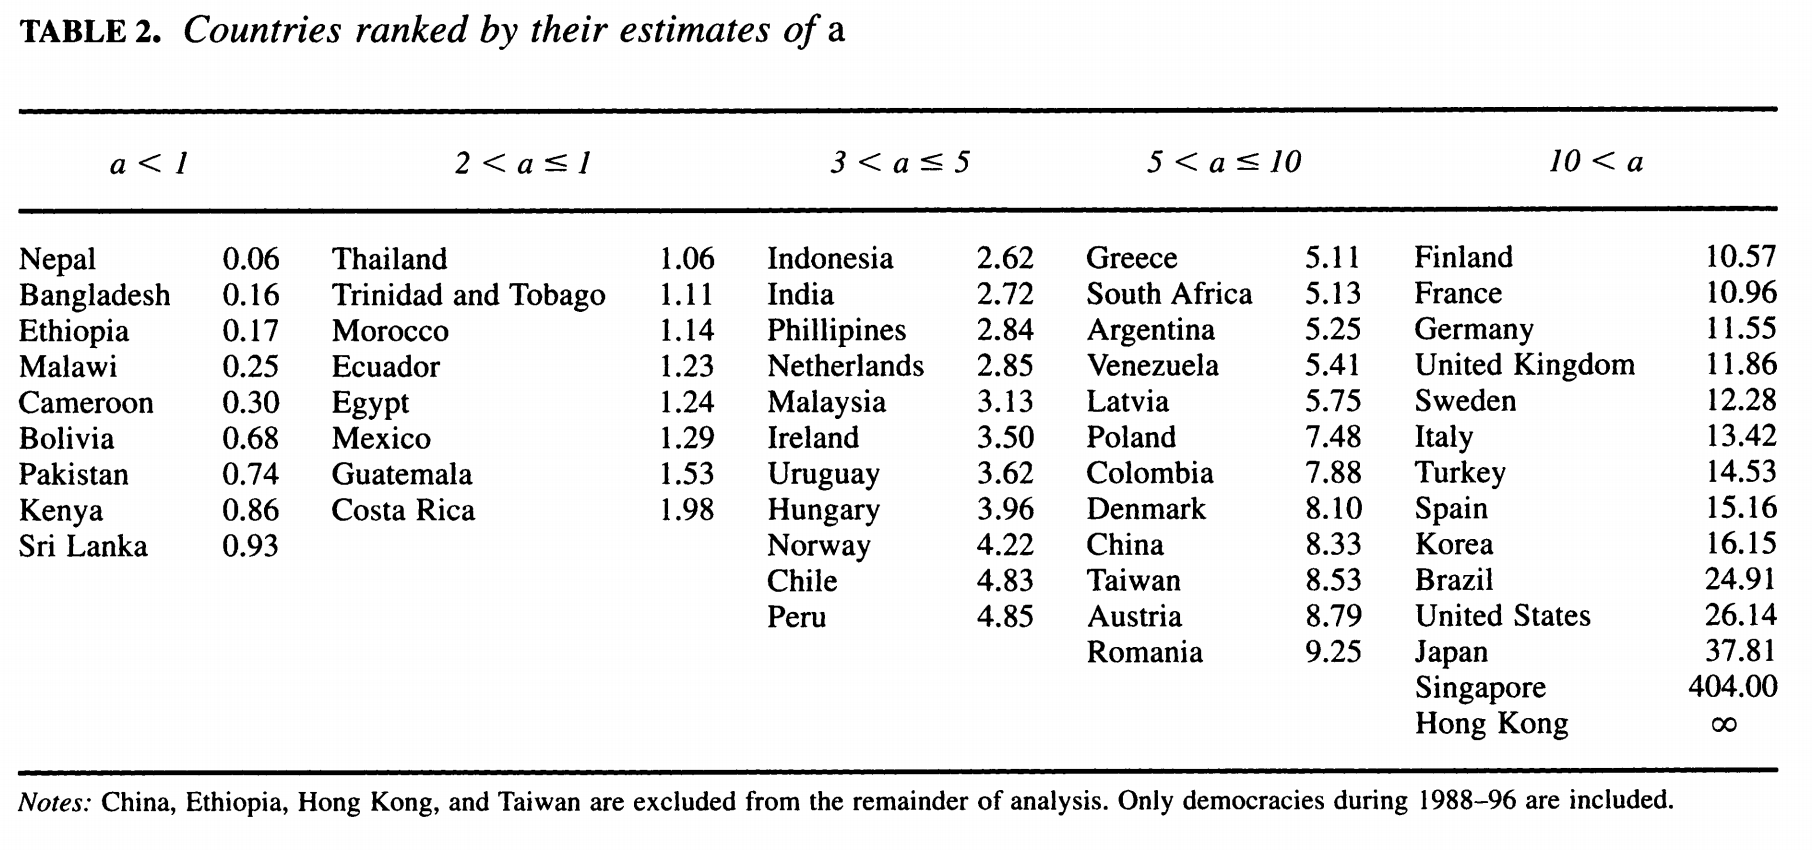
\includegraphics[width=0.9\textwidth]{table.png}
\end{figure}

\vspace{-1em}
\centering \footnotesize From Gawande, Krishna, \& Olarreaga (2009). 
\end{frame}

\begin{frame}{What makes a ``good'' formal theory paper?}

\Large 

\begin{tcolorbox}
Discuss!
\end{tcolorbox}

\normalsize
Things to consider:
\begin{itemize}
\item What do formal models give us that other forms of theorizing don't?
\item What are the limitations of formal models?
\item How do you respond to someone who says: ``assumption $X$ is empirically false, so this model is obviously useless'' ?
\item Which paper from this course did you find the most interesting? Why?
\end{itemize}

\end{frame}

\begin{frame}{What makes a ``good'' formal theory paper?}

\Large 
This is obviously highly-subjective... but most of my favourite papers fall into two categories:

\begin{enumerate}
\item Rigorous \alert{proof} of an existing intuition
\pause
\item Rigorous \alert{debunking} of an existing intuition
\end{enumerate}
\end{frame}

\begin{frame}{Type 1: Rigorous proof of an existing intuition}

\begin{outline}
\1 Meltzer \& Richard (1981)
\2 Obvious intuition: high earners prefer lower tax rates
\pause 
\2 \alert{But}: need to endogenize labor supply!

\pause 

\vspace{1em}
\1 Roemer (1998)
\2 Obvious intuition: bundling issues changes who the decisive voter is
\pause 
\2 \alert{But}: need to come up with a new solution concept (PUNE) for multidimensional space!

\end{outline}

\end{frame}

\begin{frame}{Type 2: Rigorous debunking of an existing intuition}

\begin{outline}
\1 Ashworth, Bueno de Mesquita, Friedenberg (2018)
\2 Obvious intuition: rational voters do not punish incumbents for random shocks (like natural disasters)
\pause
\2 \alert{But}: random shocks give voters the opportunity to learn new information about the incumbent! 

\pause 

\vspace{1em}
\1 Wolton (2019)
\2 Obvious intuition: biased media are bad for democracy
\pause
\2 \alert{But}: media environment affects politicians' behavior as well as voters' information! Biased media reduces ability to select good types but increases ability to control bad types.

\end{outline}

\end{frame}



\end{document}
